\documentclass[10pt]{article}
\usepackage{graphicx}
\DeclareGraphicsExtensions{.pdf,.png}
\graphicspath{{./figures/}}
\usepackage{url}
\usepackage{epsfig} 
\usepackage{amssymb}
\usepackage{amsmath}
\usepackage{amsfonts}
\usepackage{floatflt}
\setcounter{secnumdepth}{5}
\setcounter{tocdepth}{5}


\setlength{\oddsidemargin}{0in}   % 10pt is 1.875 for margins in latex
\setlength{\evensidemargin}{0in}
\setlength{\textwidth}{6.5in}
\setlength{\textheight}{9in}
\setlength{\topmargin}{-0.5in}

\newcommand{\ignore}[1]{}

\thispagestyle{empty}
\begin{document}
\date{}

\title{Governance of Web APIs in Modern Cloud Computing Environments}

\author{Hiranya Jayathilaka\\
Department of Computer Science\\
Univ. of California, Santa Barbara, CA\\
Email: hiranya@cs.ucsb.edu
}
\maketitle

\section{Introduction}
Cloud computing is fostering a model of 
application development that combines authored code with functionality
provided by extant, curated web services.  Consumer-targeting applications 
(particularly those designed for mobile platforms and the WWW) interact with highly
scalable and reliable ``back-end'' web services that are deployed
in well-connected, secure data centers.  In addition, enterprise
Information Technology (IT) strategies are focusing on 
exposing their {\em digital assets} as
web services for consumption
by their employees via internal corporate applications or
by their customers via software and data ``as-a-service''.

This rapidly proliferating model of application development and IT operation
is designed to scale, both in the number of applications, 
and in the number of web services that must be
hosted and curated.  Each web service exports one or more Application Programming
Interfaces (APIs) that must be accessible by users, applications, and/or
other services.
Because applications encode their internal logic in terms of
remote ``calls'' to curated services,
these APIs define functional boundaries that must be incorporated into the
application architecture.  

%APIs also define the boundaries between IT's management responsibility and the
%customer base it serves.  
%Applications and users ``see'' the APIs and not the
%complexity of the services that implement them (which may, in fact, be held as
%trade secrets).  Thus, the APIs have become the critical value-carrying 
%digital asset in many sectors of the new digital economy.

From an IT management perspective, the vast collection of web APIs must be
governed as critical infrastructure components or else ``client'' applications
will fail to meet their service-level agreements (SLAs)
or become unavailable altogether, due to the changes and faults in APIs.  
%That is, APIs have become separate digital artifacts that 
%must be managed by IT to ensure operational functionality.
%Modern software management strategies, such as DevOps,
%require teams comprised of both developers and sysadmins to develop, 
%deploy, and manage web services
%that IT must curate and oversee.  In the case of Google or Amazon, these
%teams number in the hundreds and the APIs that their services export in the
%thousands.  
Further, these services often make API calls to each other 
creating dependencies between APIs that must be carefully managed.
Moreover, the APIs have a software life cycle that is
independent and longer than the life cycle of the services themselves. 
As technological improvements make better service implementations possible, IT
management must upgrade these services while keeping the APIs unchanged.
Similarly, as new API versions emerge to increase functionality, backward
compatibility must be maintained in a way that takes into
account the strategic objectives of the organization.  As an organization
grows under this new model, the costs associated with
incorrectly managing APIs grow as well.

Today's cloud computing platforms severely lag behind in 
API governance. Typical cloud environments impose certain restrictions
on applications and web services in order to guarantee scalability
and high availability (e.g. Google App Engine prevents applications from accessing
the file system). 
However, they do not prevent the developers from violating
software development policies and maintenance best practices. 
Consequently, developers often violate naming and versioning conventions
when naming APIs and other digital assets, take dependencies
on incorrect or deprecated APIs, and very often end up re-implementing program logic
from the scratch instead of reusing extant APIs that provide the required functionality.
This lack of API governance also leads to many security vulnerabilities (e.g. DoS attacks
by malicious or poorly coded clients), violations of IP rights and licensing terms, and in
some cases even financial losses. Web APIs also play a key role in SLA
management and enforcement. Ideally, any public API should be exposed with a well-defined
SLA detailing its performance and quality of service characteristics. Without proper means
of API governance, developers that host services in cloud settings have no way of enforcing
competitive SLAs on their APIs, or even getting a thorough idea of what kind of SLAs
their services can uphold. Today, developers have to perform a lot of offline
and online testing to learn the performance characteristics of their APIs which is tedious and
time-consuming. Furthermore developers often have to be content with basic SLA monitoring 
as opposed to comprehensive SLA enforcement. Moreover, the general deficiency in
automated mechanisms for developing, analyzing and reasoning 
about web APIs in cloud environments
is a strong inhibitor of cloud adoption by many developers and enterprises.

My research focuses on designing and implementing systems for facilitating 
strong API governance as a cloud-native feature. With this research, API
governance will no longer be an afterthought or a feature poorly layered on
top of a computing cloud. Rather, it would be supported as a capability built into
the cloud that is hosting the APIs and the cloud management
tools used to develop APIs. 
In a cloud-based IT context, APIs must be governed by
policies that are defined by the organization to ensure predictable and
economic operation of the web services hosted by the cloud. Additionally
there should be automated mechanisms in place for easily developing new
APIs, discovering existing APIs, analyzing the syntactic and semantic features
of APIs, and porting applications across APIs. My research will make 
it easier for developers to consume, mix and match APIs to create powerful
applications, while adhering to tried and tested software development and 
maintenance best practices. They will be able to quickly and easily understand
the QoS properties of APIs and enforce competitive SLAs through the cloud
with clear and accurate confidence levels. My plan is to
\begin{itemize}
%\item develop new {\bf policy specification languages for web
%services} that
%enables governance enforcement during service development, 
%and at runtime,
\item develop a distributed {\bf platform for enforcing IT 
management policies} governing
web APIs when operating at scale in cloud settings,
\item develop automated mechanisms for discovering, analyzing, comparing and reasoning
about web APIs, in order to {\bf simplify the API-based development model} and
the inevitable process of porting applications across different APIs or API versions,
\item develop methods for {\bf automated QoS and performance analysis} of web services
using static analysis, simulations and runtime monitoring in order
to formulate and enforce competitive SLAs for APIs hosted in clouds, and,
\item focus on the {\bf API software components} as the boundary between 
IT-managed
service implementations and client users, software applications, and other
services.
\end{itemize}

My research is based on a number of other prominent research areas in computer
science including programming languages, program analysis and verification, 
distributed systems and software engineering. The proposed policy enforcement
platform for clouds motivates new research on innovative new ways of using existing
distributed consensus, scalability and high availability techniques. It also calls for
more research in novel policy specification languages that
are easier to understand (for policy authors), analyze and execute in cloud settings.
Automated QoS and performance analysis requires more research in using
static analysis methods (e.g. abstract interpretation, WCET analysis etc.), system modeling,
and simulations for analyzing a wide range of services deployed in modern cloud platforms.
Automated mechanisms for discovering and analyzing web APIs require more research
in specifying the syntactic and semantic features of APIs in a machine-readable way
and processing such specifications efficiently. Above all, since the primary target of this
work are cloud platforms, there needs to be a strong focus towards making all these 
proposed mechanisms scale to handle thousands of APIs, policies, client applications and users.

\subsection{Outcomes and Assessment}

The outcome of this research plan,
I believe, will be new advances in services computing, IT management, cloud
platform computing, and API policy enforcement and SLA management.
If successful, the research will be transformative as it
enables scalable management of the services that form the
bulk of cloud workloads.

In addition,
as a cloud systems researcher, I intend to use open source, on-premise clouds (AppScale
and Eucalyptus) to serve research and educational artifacts (data sets, demos and test applications, 
code repositories, etc.) to my colleagues, 
and the wider research community.  Another measure of success will
be the degree to which my research reduces the management burden that results from
the scale and speed that these systems require.

Finally, I plan to make my systems, tools and mechanisms available as persistent software artifacts to
the wider research community and to monitor its uptake.  Because of their design
and their use of open source cloud technologies, results of my research will be readily available
to researchers and educators who wish to develop new artifacts and curricula
for cloud computing. 

\section{Research Context: API-driven Development Model in the Cloud}
As scalable information technology evolves to a more cloud-like model,
{\em digital assets} (code, data, software environments, and technologies) 
are increasingly integrated into applications by developers 
as web-accessible services.
This application development model facilitates code reuse and eases the 
assembly of complex systems thereby greatly improving programmer productivity
over non-service-oriented methodologies~\cite{Dan:2008:SSR:1370916.1370923}. 
By composing an application from existing services that 
encapsulate common yet complicated tasks such as
database access, logging, and security, or the audited access of useful 
digital assets, application developers are able  
to work at a higher level of abstraction, employ any programming 
language they choose, leverage the work, testing, and quality
assurance of others, and thus innovate faster.  

\begin{floatingfigure}[rb]{2.8in}
\vspace{-0.1in}
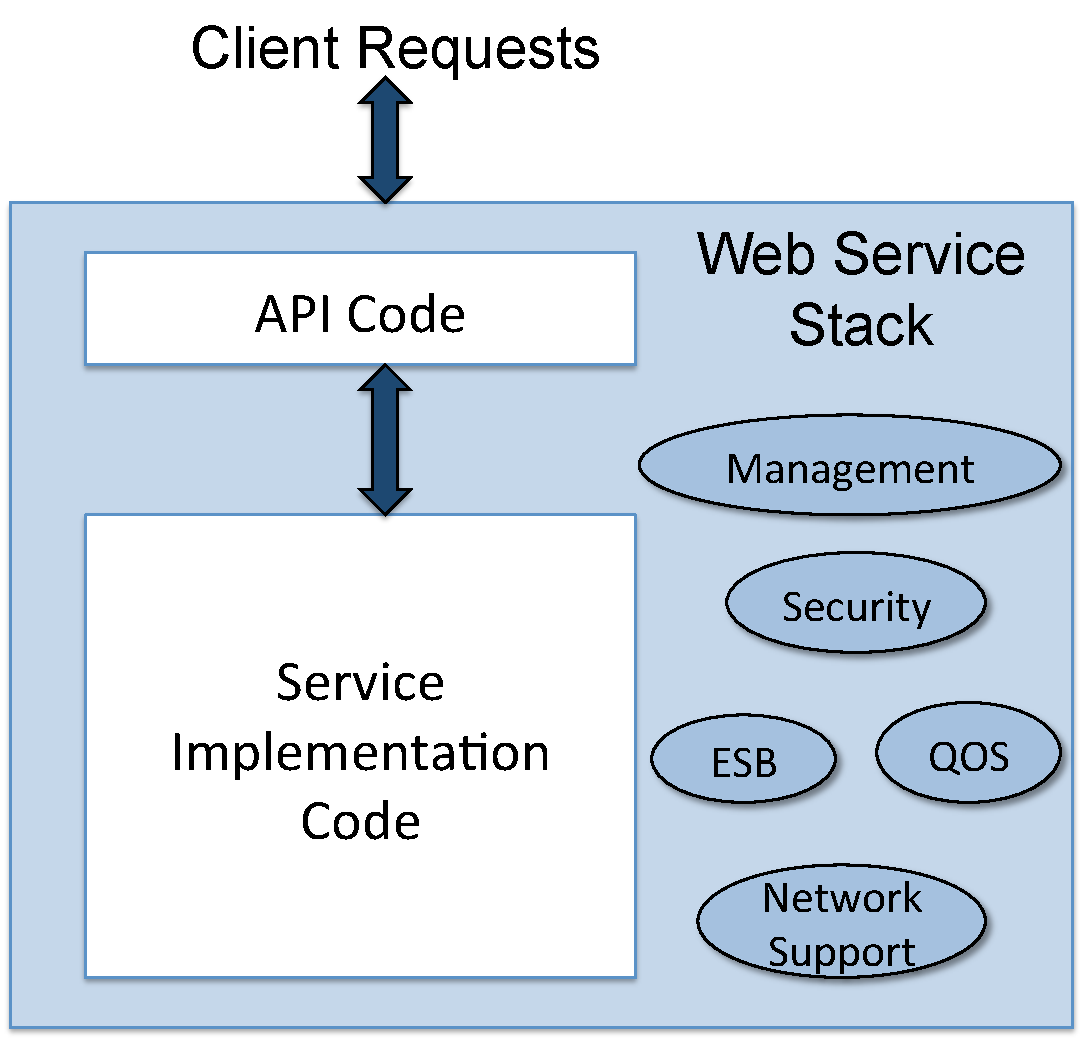
\includegraphics[scale=.34]{stack}
\vspace{-0.08in}
\caption{Web Service Software Components\label{fig:ws-arch}}
\end{floatingfigure}
Production web services consist of three components: API code, service
implementation code, and a web service ``stack'' that implements a container
for combining and deploying the API and service implementation
together ({\em c.f.} Figure~\ref{fig:ws-arch}).
Clients contact the web service container which routes requests to the
API code.  The container implements common functions such as 
service management (registration, description, discovery), a service
bus (ESB), security policy enforcement, and networking support, among other 
functions that both API and service implementation code access.
Service clients in production settings can be 
external, i.e., customers of the enterprise, or internal, i.e., employees of 
the organization.  These clients access the services via user 
interfaces (e.g. via a browser) or programmatically via web applications 
or other services. 

Increasingly, IT organizations are tasked with deploying and 
maintaining web services as software infrastructure components, hosted in a
shared cloud platform ({\em i.e.} in a way analogous to the manner in which they
would deploy and maintain a piece of shared physical infrastructure).  
To achieve economies of scale, these services are shared (in a controlled
way) among the widest possible set of users and client applications.  Indeed,
it is the possibility of Internet-scale sharing that makes this model
attractive from an IT management perspective. As a consequence we 
are witnessing an explosion of web APIs on the Internet today. ProgrammableWeb,
the popular online API registry currently boasts over 12,000 registered APIs and
a near exponential growth rate since 2006.

The modular design of web services inherently separates API, 
service implementation, and container. However, only 
the service implementation and the container is under complete
control of IT. External clients access APIs independently from IT.
Even internally developed client applications may be too numerous and
constantly evolving for IT to track or control given
potentially tens or hundreds of engineering teams and hundreds or 
thousands of APIs.  That is, the decoupling of the API from the 
other components of the web service provides many programmer
benefits, but it also introduces several IT management challenges 
at production scales. 

The confluence of application concerns ({\em e.g.} 
application functionality and productivity) with IT 
concerns ({\em e.g.} life cycle management, security, 
cost management) has led to new organizational approaches such as
DevOps.  However, 
the technologies that have been developed
to date address the core API
governance challenges incompletely, if at all. 
In particular, new research and technology is needed 
to provide scalable and unified automation to the problem
of implementing and enforcing consistent governance for APIs. 
By using automation to ensure consistency, our goal is to alleviate the 
labor burden associated with uniform policy implementation and SLA enforcement.  
Consistent policy implementation across APIs will reduce (and perhaps
eliminate) some of the cost scaling factors that the need for API governance
introduces.  Thus, at the same time automation ensures cost-saving
consistency, we believe it will also lead to productivity gains for 
IT management through reduced labor burden.

To my knowledge, there is no extant system that automates governance and
SLA enforcement across the life cycle
of an API, across diverse categories of policies, for web
APIs in cloud environments simply and scalably.  The goal of my work is to investigate 
new research and to develop
new technologies that do so for the next generation of service ecosystems.

\end{document}
